\documentclass{article}

\usepackage{fancyhdr}
\usepackage[parfill]{parskip}
\usepackage{tikz}

\pagestyle{fancyplain}

\author{Todd Davies}
\title{3.2.4 Cells and substances}
\date{\today}

\begin{document}

\rhead{3.2.4 Cells and substances}
\lhead{\today}

\maketitle

\section*{Haemoglobin}
\thispagestyle{empty}

\subsection*{What's haemoglobin?}

Haemoglobin, mainly found in red blood cells, is a large protein with a
\marginpar{Proteins with quaternary structures are made of more than one chain
of amino acids joined together}{\it quaternary structure} that is able to absorb
oxygen. Different species of organisms have different types of haemoglobin (and
some have no haemoglobin at all).

\subsection*{Oxygen association}

Haemoglobin has a high affinity for oxygen. One haemoglobin molecule {\it can
carry four oxygen molecules}. When oxygen is combined to haemoglobin, the
resulting compound is called {\it oxyhaemoglobin}. Oxygen dissasociates from
haemo\-globin with the same ease that it associates with it, the reaction is
reversable.

\marginpar{The partial pressure of a gas is a mesaure of it's concentration.}

Oxygen loads onto haemoglobin to form oxyhaemoglobin when there's a high $pO_2$.
Oxyhaemoglobin unloads it's oxygen when there's a low $pO_2$.

In the lungs, the alveoli have a high $pO_2$, so oxygen is loaded onto the
haemoglobin. Conversely, when cells respire, they use up oxygen, lowering the
$pO_2$ in the process. This causes oxyhaemoglobin to unload its oxygen.

\subsection*{Dissociation curves}

Dissociation curves show how saturated haemoglobin is with oxygen at any given
partial pressure. It is a graph of \% saturation on the y axis, and partial
pressure on the x axis. The curve is a sigmoid (S) shape.

When haemoglobin combines with its first oxygen molecule, the shape of the
protein changes, making the next oxygen molecule easier to join (so the gradient
increases in the middle of the curve). However, as the haemoglobin becomes more
saturated, it becomes harder for oxygen molecules to join and the gradient of
the curve levels off (at high $pO_2$).

Because of the sigmoid shape of the curve, a small change in $pO_2$ can cause a
big change in the amount of oxygen carried.

\subsubsection*{Carbon dioxide affects the dissociation curve}

\marginpar{This is called the Bohr effect} At a high $pCO_2$, haemoglobin
releases it's oxygen more readily. This ensures that when cells are respiring
quickly (and releasing lots of $CO_2$ as a bi- product) that they get enough
oxygen to continue respiring aerobically.

Because oxygen unloads more readily at high partial pressures of $CO_2$, the
dissociation curve shifts down and to the right.

\subsubsection*{The dissociation curve varies between organisms}

As you might expect, differences in the gene that codes for haemoglobin in
different organisms create differences in the actual protein itself. This means
that the dissociation curve for two organisms is often dissimilar.

As a general rule:

\begin{itemize}

	\item Organisms that live in environments with a {\bf low oxygen
	concentration} have haemoglobin with a {\bf high affinity} for oxygen.
	Their dissociation curves are {\bf shifted to the left}. (e.g. worm)

    \item Organisms that are {\bf very active} and have a high demand for oxygen
	have haemoglobin with a {\bf low affinity} for oxygen. Their dissociation
	curves are {\bf shifted to the right}. (e.g. hawk)

\end{itemize}

\section*{Carbohydrates}

\subsection*{What's a carbohydrate?}

A carbohydrate is a long chain molecule made from many monosaccharides strung
together. Examples of monosaccharides include glucose ($\alpha$ and $\beta$),
and fructose.

\begin{center}
	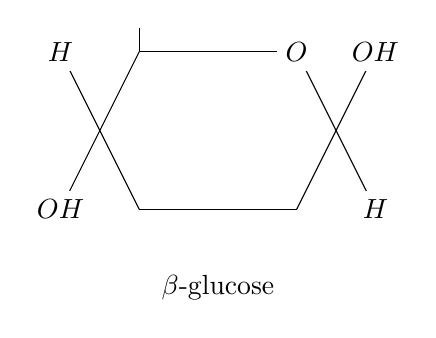
\begin{tikzpicture}
		
			\draw [-] (0,2) -- (1,0);
			\draw [-] (0,0) -- (1,2);

			\draw [-] (1,2) -- (1,2.3);

			\draw [-] (1,0) -- (3,0);
			\draw [-] (1,2) -- (3,2);

			\draw [-] (3,0) -- (4,2);
			\draw [-] (3,2) -- (4,0);
		
			\node[fill=white] at (0,2) {$H$};
			\node[fill=white] at (0,0) {$OH$};
		
			\node[fill=white] at (3,2) {$O$};

			\node[fill=white] at (4,2) {$OH$};
			\node[fill=white] at (4,0) {$H$};

			\node[fill=white] at (2,-1) {$\beta$-glucose};

	\end{tikzpicture}
\end{center}


\subsubsection*{Condensation reactions}

In a condensation reaction, two monosaccharides join together to form part of a
polysaccharide chain and a {\bf water molecule is released}.

When two sugars join, they are said to be linked by a {\bf glycosidic bond}.

In a glycosidic bond, a hydrogen from one glucose molecule and a hydroxide from
another are removed, and the two molecules are joined with an oxygen atom.

Here are two monosaccharides, the pink highlighted symbols are going to be
removed.

\begin{center}
	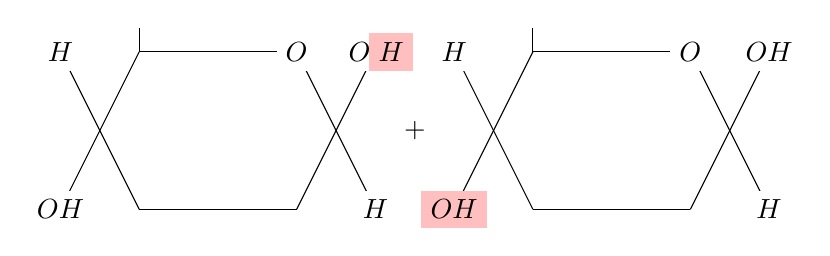
\begin{tikzpicture}

			\draw [-] (0,2) -- (1,0);
			\draw [-] (0,0) -- (1,2);

			\draw [-] (1,2) -- (1,2.3);

			\draw [-] (1,0) -- (3,0);
			\draw [-] (1,2) -- (3,2);

			\draw [-] (3,0) -- (4,2);
			\draw [-] (3,2) -- (4,0);
		
			\node[fill=white] at (0,2) {$H$};
			\node[fill=white] at (0,0) {$OH$};
		
			\node[fill=white] at (3,2) {$O$};

			\node[fill=white] at (3.8,2) {$O$};
			\node[fill=pink] at (4.2,2) {$H$};
			\node[fill=white] at (4,0) {$H$};

			\node[fill=white] at (4.5,1) {$+$};

			\draw [-] (5,2) -- (6,0);
			\draw [-] (5,0) -- (6,2);

			\draw [-] (6,2) -- (6,2.3);

			\draw [-] (6,0) -- (8,0);
			\draw [-] (6,2) -- (8,2);

			\draw [-] (8,0) -- (9,2);
			\draw [-] (8,2) -- (9,0);
		
			\node[fill=white] at (5,2) {$H$};
			\node[fill=pink] at (5,0) {$OH$};
		
			\node[fill=white] at (8,2) {$O$};

			\node[fill=white] at (9,2) {$OH$};
			\node[fill=white] at (9,0) {$H$};

	\end{tikzpicture}
\end{center}

Here is a polysaccharide, joined with a glycosydic bond. The pink $H_2O$
molecule has been removed.

\begin{center}
	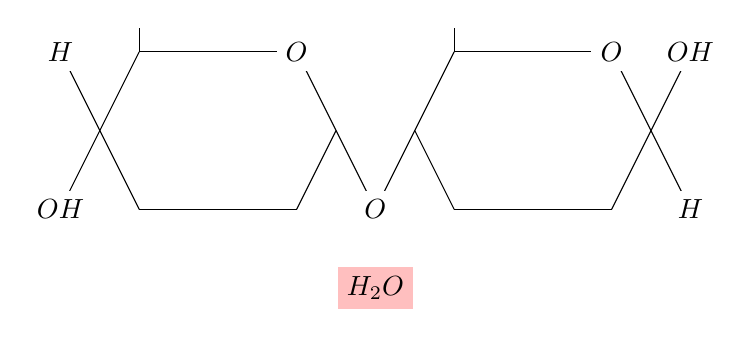
\begin{tikzpicture}

			\draw [-] (0,2) -- (1,0);
			\draw [-] (0,0) -- (1,2);

			\draw [-] (1,2) -- (1,2.3);

			\draw [-] (1,0) -- (3,0);
			\draw [-] (1,2) -- (3,2);

			\draw [-] (3,0) -- (3.5,1);
			\draw [-] (3,2) -- (4,0);
		
			\node[fill=white] at (0,2) {$H$};
			\node[fill=white] at (0,0) {$OH$};
		
			\node[fill=white] at (3,2) {$O$};

			\draw [-] (4,0) -- (5,2);
			\draw [-] (4.5,1) -- (5,0);

			\draw [-] (5,2) -- (5,2.3);

			\draw [-] (5,0) -- (7,0);
			\draw [-] (5,2) -- (7,2);

			\draw [-] (7,0) -- (8,2);
			\draw [-] (7,2) -- (8,0);

			\node[fill=white] at (7,2) {$O$};

			\node[fill=white] at (8,2) {$OH$};
			\node[fill=white] at (8,0) {$H$};

			\node[fill=pink] at (4, -1) {$H_2O$};

			\node[fill=white] at (4,0) {$O$};

	\end{tikzpicture}
\end{center}

\subsubsection*{Polysaccharides}

There are three important polysaccharides to know about:

\begin{itemize}

	\item {\bf Starch} is the main energy store in plants. Excess glucose is
	converted to starch for times of need. It's a mixture of two
	polysaccharides of {\it alpha-glucose}, amylose and amylopectin.

	\begin{itemize}

		\item Amylose is a long unbranched chain. This means it's very compact,
		but also slow to break down.

		\item Amlyopectin is a long, branched chain. The branches allow enzymes
		to break down the molecule quickly to release glucose fast.

	\end{itemize}

	\item {\bf Glycogen} is the main energy store in animals. It is similar to
	amlyopectin (and uses alpha-glucose too), but much more highly branched
	which allows glucose to be released very rapidly. It is a relativly compact
	molecule.

	\item {\bf Cellulose} is what makes up the cell wall of plants. It is a long
	unbranched chain of beta-glucose. The bonds between the glucose molecules
	are straight, so the chains are straight, allowing them to be linked
	together by hydrogen bonds, forming strong {\it microfibrils}. They provide
	structural support for cells.

\end{itemize}

\end{document}